\documentclass[11pt]{article}

\usepackage{pablo}
\usepackage{pablo-listings}
\usepackage[a5paper,margin=0.7cm]{geometry}
\usepackage{eurosym}
\usepackage{multicol}

\pagestyle{empty}

\begin{document}

\begin{center}
  Corrigé

  \textsc{Systèmes et Droites}
\end{center}

\begin{exercice}[Équations de droites]~

  \begin{center}
    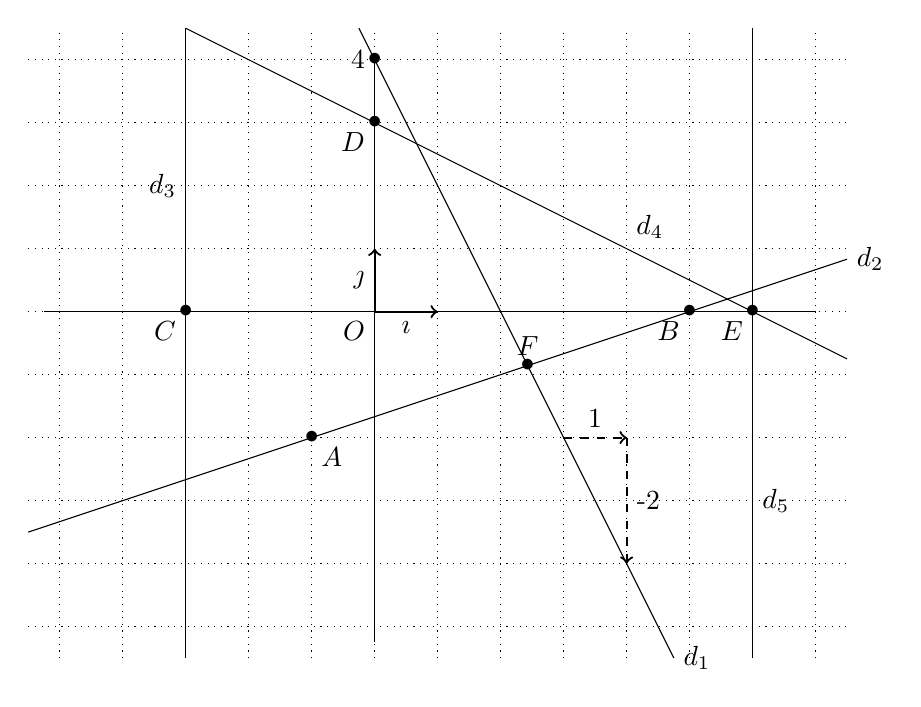
\begin{tikzpicture}[scale=0.8]
      \shorthandoff{:}
      % Quadrillage
      \draw[color=black,step=1,dotted] (-5.5,-5.5) grid (7.5,4.5);

      % Repère
      \draw (-5.25,0) -- (7,0);
      \draw[thick,->] (0,0) -> (1,0) node[midway,below] {$\vecteur\imath$};
      \draw (0,-5.25) -- (0,4);
      \draw[thick,->] (0,0) -> (0,1) node[midway,left] {$\vecteur\jmath$};
      \draw (0,0) node[below left] {$O$};

      %     % Objets
      \draw[smooth,samples=100,domain=-0.25:4.75] plot(\x,{-2*(\x)+4}) node[right] {$d_1$};
      \draw[smooth,samples=100,domain=-5.5:7.5] plot(\x,{1/3*(\x)-5/3}) node[right] {$d_2$};
      \draw (-3,-5.5) -- (-3,4.5);
      \draw (-3,2) node[left] {$d_3$} ;

      % Solutions
      \draw[smooth,samples=100,domain=-3:7.5] plot(\x,{-1/2*(\x)+3});
      \draw (6,-5.5) -- (6,4.5);
      \draw (4,1) node[above right] {$d_4$} ;
      \draw (6,-3) node[right] {$d_5$} ;
      \draw (0,4) node{$\bullet$} node[left]{4};
      \draw[thick,dashed,->] (3,-2) -- (4,-2) node[midway,above]{1};
      \draw[thick,dashed,->] (4,-2) -- (4,-4) node[midway,right]{-2};
      \draw (-1,-2) node{$\bullet$} node[below right]{$A$};
      \draw (5,0)   node{$\bullet$} node[below left]{$B$};
      \draw (-3,0)   node{$\bullet$} node[below left]{$C$};

      \draw (0,3) node{$\bullet$} node[below left]{$D$};
      \draw (6,0) node{$\bullet$} node[below left]{$E$};
      \draw (17/7,-6/7) node{$\bullet$} node[above]{$F$};
    \end{tikzpicture}
  \end{center}

  \begin{enumerate} 
    \item \emph{Donner les équations des droites $d_1$, $d_2$ et $d_3$. }
      \begin{description}
        \item[$d_1$ :] Le coefficient directeur et l'ordonnée à l'origine peuvent se lire sur le graphique : $d_1:y=-2x+4$.
        \item[$d_2$ :] Prenons les points $A(-1,-2)$ et $B(5,0)$ appartenant à la droite $d_2$. Le coefficient directeur de la droite est $a=\frac{y_B-y_A}{x_B-x_A}=\frac{0-(-2)}{5-(-1)}=\frac{2}{6}=\frac{1}{3}$. L'équation de la droite est donc de la forme $y=\frac{1}{3}x+b$. Or $A\in d_2$, donc $y_A=\frac{1}{3}x_A+b$, c'est-à-dire $-2=\frac{1}{3}\times(-1)+b$, d'où $b=-\frac{5}{3}$. Ainsi l'équation de $d_2$ est $y=\frac{1}{3}x-\frac{5}{3}$.
        \item[$d_3$ :] La droite est parallèle à l'axe des ordonnées, donc son équation est de la forme $x=c$. On prend un point appartenant à la droite, par exemple $C(-3,0)$. Son absicce est $-3$, donc l'équation de la droite est $x=-3$.
      \end{description}
    \item \emph{Déterminer les coordonnées du point d'intersection de $d_1$ et $d_2$. }
      On résout le système suivant,rassemblant les équations des droites $d_1$ et $d_2$ : $\systeme{y=-2x+4}{y=\frac{1}{3}x-\frac{5}{3}}$. On commence par soustraire les deux lignes.
      \setlength{\columnsep}{2cm}
      \begin{multicols}{2}
        $\systeme{y-y=-2x+4-(\frac{1}{3}x-\frac{5}{3})}{y=\frac{1}{3}x-\frac{5}{3}}$

        $\systeme{0=-2x+4-\frac{1}{3}x+\frac{5}{3}}{y=\frac{1}{3}x-\frac{5}{3}}$

        $\systeme{0=-\frac{7}{3}x+\frac{17}{3}}{y=\frac{1}{3}x-\frac{5}{3}}$

        $\systeme{x=\frac{17}{7}}{y=\frac{1}{3}\frac{17}{7}-\frac{5}{3}}$

        $\systeme{x=\frac{17}{7}}{y=-\frac{6}{7}}$

        Donc le point d'intersection de $d_1$ et $d_2$ est le point $F$ de coordonnées $\left(\frac{17}{7},-\frac{6}{7}\right)$.
      \end{multicols}
    \item \emph{Tracer, sur le graphique précédent,
      les droites d'équations $y = -\frac{1}{2}x+3$ et $x = 6$. }
      \begin{description}
        \item[$d_4$ :] $-\frac{1}{2}\times0+3=3$, donc $D(0,3)\in d_4$ ; $-\frac{1}{2}\times6+3=0$, donc $E(6,0)\in d_4$.
        \item[$d_5$ :] Puisque l'équation est de la forme $x=6$, sa représentation est une droite verticale d'abscisse $6$.
      \end{description}
  \end{enumerate}
\end{exercice}

\begin{exercice}[Vecteurs et droites]~

  \begin{center}
    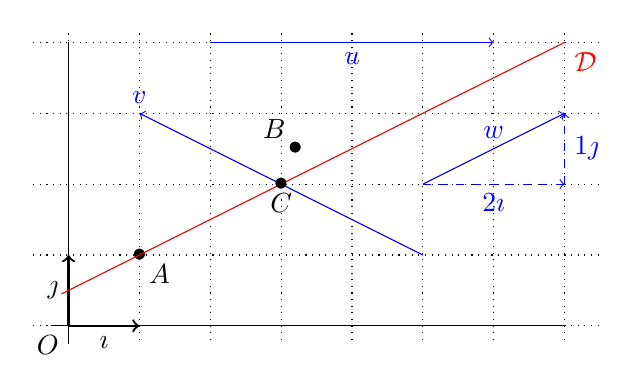
\begin{tikzpicture}[scale=0.9]
      % Quadrillage
      \draw[color=black,step=1,dotted] (-.5,-.2) grid (7.5,4.2);

      % Repère
      \draw (-.25,0) -- (7,0);
      \draw[thick,->] (0,0) -> (1,0) node[midway,below] {$\vecteur\imath$};
      \draw (0,-.25) -- (0,4);
      \draw[thick,->] (0,0) -> (0,1) node[midway,left] {$\vecteur\jmath$};
      \draw (0,0) node[below left] {$O$};

      % Objets
      \draw (1,1) node{$\bullet$}node{$\bullet$}  node[below right] {$A$};
      \draw[color=blue,->] (2,4) -- (6,4) node[midway,below]{$\vecteur{u}$};
      \draw[color=blue,->] (5,1) -- (1,3) node[above]{$\vecteur{v}$};

      % Solutions
      \draw[color=blue,->] (5,2) -- (7,3) node[midway,above]{$\vecteur{w}$};
      \draw[dashed,color=blue,->] (5,2) -- (7,2) node[midway,below]{$2\vecteur\imath$};
      \draw[dashed,color=blue,->] (7,2) -- (7,3) node[midway,right]{$1\vecteur\jmath$};
      \draw[color=red,domain=-0.1:7] plot (\x,{\x/2+.5}) node[below right]{$\cal D$};
      \draw (3,2) node{$\bullet$}node{$\bullet$}  node[below] {$C$};
      \draw (3.2,2.5) node{$\bullet$}node{$\bullet$}  node[above left] {$B$};
    \end{tikzpicture}
  \end{center}

  \begin{enumerate}
    \item Les coordonnées sont $A(1,1)$, $\vecteur{u}(4,0)$ et $\vecteur{v}(-4,2)$.
    \item $\vecteur w=\vecteur u +\frac{1}{2}\vecteur v$. Les coordonnées de $\frac{1}{2}\vecteur v$ sont $\coord{\frac{1}{2}\times-4}{\frac{1}{2}\times2}$, c'est-à-dire $\coord{-2}{1}$. Donc les coordonnées de $\vecteur w$ sont $\coord{4+(-2)}{0+1}$, c'est-à-dire $\coord{2}{1}$.
    \item \begin{enumerate}
        \item \emph{Tracer la droite $\cal D$ de vecteur directeur $\vecteur w$ passant par $A$.} Voir sur le graphique : on trace le vecteur $\vecteur w$, puis on trace la droite \og{} parallèle \fg{} à ce vecteur passant par $A$.
        \item \emph{Le point $B(3,2;2,5)$ appartient-il à la droite $\cal D$ ?}
          \emph{Vérifier votre réponse sur le graphique.} On commence par calculer l'équation de la droite $\cal D$. Le point $C(3,2)$ appartient à la droite $\cal D$ (il a été obtenu par une translation de $A$ par le vecteur $\vecteur w$, donc ses coordonnées sont la somme des coordonnées de $A$ et $\vecteur w$). Le coefficient directeur de la droite est donc $a=\frac{y_C-y_A}{x_C-x_A}=\frac{2-1}{3-1}=\frac{1}{2}$. L'équation est donc de la forme $y=\frac{1}{2}x+b$. Puisque le point $A$ appartient à $\cal D$, on a $y_A=\frac{1}{2}x_A+b$, donc $1=\frac{1}{2}\times1+b$, donc $b=\frac{1}{2}$. L'équation de $\cal D$ est donc $y=\frac12x+\frac12$.

          Vérifions si le point $B$ appartient à $\cal D$ : $\frac{1}{2}\times x_B+\frac{1}{2}=\frac{1}{2}\times3,2+\frac{1}{2}=2,1$. Or $2,1\neq x_B$, donc $B$ n'est pas sur la droite $\cal D$.

          Graphiquement, on place le point $B$ sur le graphique, et on observe qu'il n'est pas sur la droite.
      \end{enumerate}
    \item \begin{enumerate}
        \item L'algorithme vérifie si le point donc les coordonnées sont données en entrées appartient ou non à la droite $\cal D$.
        \item \emph{On exécute cet algorithme avec $x=3$ et $y=2$. Qu'affiche l'algorithme ? Que peut-on en déduire ?} L'algorithme affiche \texttt{Vrai}, donc le point de coordonnées $(3,2)$ appartient à la droite $\cal D$.
      \end{enumerate}
  \end{enumerate}
\end{exercice}

\begin{exercice}[Système d'équations]~

  \begin{enumerate}
    \item Résoudre les systèmes suivants :

      \begin{multicols}{2}
      \begin{enumerate}
      \item $\systeme{y=-5-x}{y=\frac{1}{2}x+1}$

        $\systeme{y-y=-5-x-(\frac{1}{2}x+1)}{y=\frac{1}{2}x+1}$

        $\systeme{0=-\frac{3}{2}x-6}{y=\frac{1}{2}x+1}$

        $\systeme{\frac{3}{2}x=6}{y=\frac{1}{2}x+1}$

        $\systeme{x=-4}{y=\frac{1}{2}\times(-4)+1}$

        $\systeme{x=-4}{y=-1}$

        \columnbreak

      \item $\systeme{2y=x}{y=\frac{1}{2}x+1}$

      $\systeme{2y=x}{y=\frac{1}{2}x+1}$

      $\systeme{2y=x}{y=\frac{1}{2}\times2y+1}$

      $\systeme{2y=x}{y=y+1}$

      $\systeme{2y=x}{0=1}$

      Cette dernière équation n'a pas de solutions, donc l'ensemble du système n'a pas de solutions.
      \end{enumerate}
    \end{multicols}

  \item \emph{Le but de la question est de résoudre le système $(S)$ suivant :}
      \[(S)\systeme{x^2+5x-xy-10y-2y^2=0}{y=\frac{1}{2}x+1}\]
      \begin{enumerate}
        \item En développant $(x-2y)(5+x+y)$, on trouve $(x-2y)(5+x+y)=x^2+5x-xy-10y-2y^2$, donc les équations $(x-2y)(5+x+y)=0$ et $x^2+5x-xy-10y-2y^2=0$ sont équivalentes, donc les deux systèmes correspondants sont équivalents.
        \item $(x-2y)(5+x+y)=0$ si et seulement si $x-2y=0$ ou $5+x+y=0$ (c'est une équation produit), c'est-à-dire si $2y=x$ ou si $y=-5-x$. Donc le système précédent est équivalent au couple de systèmes :

          \[\systeme{2y=x}{y=\frac{1}{2}x+1} \text{ ou } \systeme{y=-5-x}{y=\frac{1}{2}x+1}\]
        \item \emph{En utilisant la première question, en déduire les solutions de $(S)$.} Le système $(S)$ étant équivalent aux deux systèmes de la question précédente, il suffit de les résoudre pour résoudre $(S)$. Cela a été fait dans la première question, et on a trouvé une seule solution $(-4,-1)$. Donc le système $(S)$ a comme unique solution $(-4,-1)$.
      \end{enumerate}
  \end{enumerate}
\end{exercice}

\begin{exercice}[Problème ouvert]
  \begin{em}
  Deux entreprises A et B emploient deux types de personnel : des cadres et des ouvriers. 
  \begin{itemize} 
    \item L'entreprise A emploie 5 cadres et 20 ouvriers. Le salaire moyen des cadres est 3020~\officialeuro{} et celui des ouvriers 1750~\officialeuro.
    \item  L'entreprise B emploie 50 personnes. Le salaire moyen des cadres est 2880~\officialeuro{} et celui des ouvriers 1650~\officialeuro.
  \end{itemize}
  Le directeur financier de l'entreprise B affirme que le salaire moyen pour l'ensemble de ses employés est supérieur à celui de l'entreprise A. Est-ce possible ? 
\end{em}

Nous pouvons déjà calculer le salaire moyen de l'entreprise $A$ : $\frac{5\times3020+20\times1750}{25}=2004$. Le salaire moyen de l'entreprise $B$ peut-il être supérieur à 2004~\officialeuro{} ?

\paragraph{Première méthode} Appelons $x$ le nombre de cadres de l'entreprise $B$, et $y$ son nombre d'ouvriers. Puisque l'entreprise a 50 employés, cela signifie que $x+y=50$, donc $x=50-y$.

\noindent La moyenne des salaires de cette entreprise est $\frac{x\times 2880+y\times 1650}{50}=\frac{(50-y)\times 2880+y\times 1650}{50}$. Nous voulons savoir si ce salaire moyen est supérieur à 2004, donc nous résolvons l'inéquation :

\[\frac{(50-y)\times 2880+y\times 1650}{50}\geq2004\]

Cela donne : $y\leq\frac{1460}{41}$, c'est-à-dire $y\leq35,6$ environ. Conclusion : si l'entreprise $B$ a moins de 35 ouvriers, son salaire moyen est plus élevé que celui de l'entreprise $A$. Donc c'est possible.

\paragraph{Seconde méthode} Supposons que l'entreprise $B$ ait 48 cadres et 2 ouvriers. Alors son salaire moyen est $\frac{48\times 2880+2\times 1650}{50}=2830,8$. Ce salaire est supérieur à celui de l'entreprise $A$, donc l'affirmation du directeur financier est possible.
\end{exercice}

\end{document}

